\documentclass{article}
\usepackage{geometry}
\geometry{a4paper,scale=0.95}
\usepackage[utf8]{inputenc}

\usepackage{amssymb}
\usepackage{graphicx}

\title{Rapport TP3}

\author{Rosine Rolande Simo Tegninko, 20183729\\
Yu Deng, 20151659}

\date{}

\begin{document}

\maketitle

\section*{Tâche 1}\\
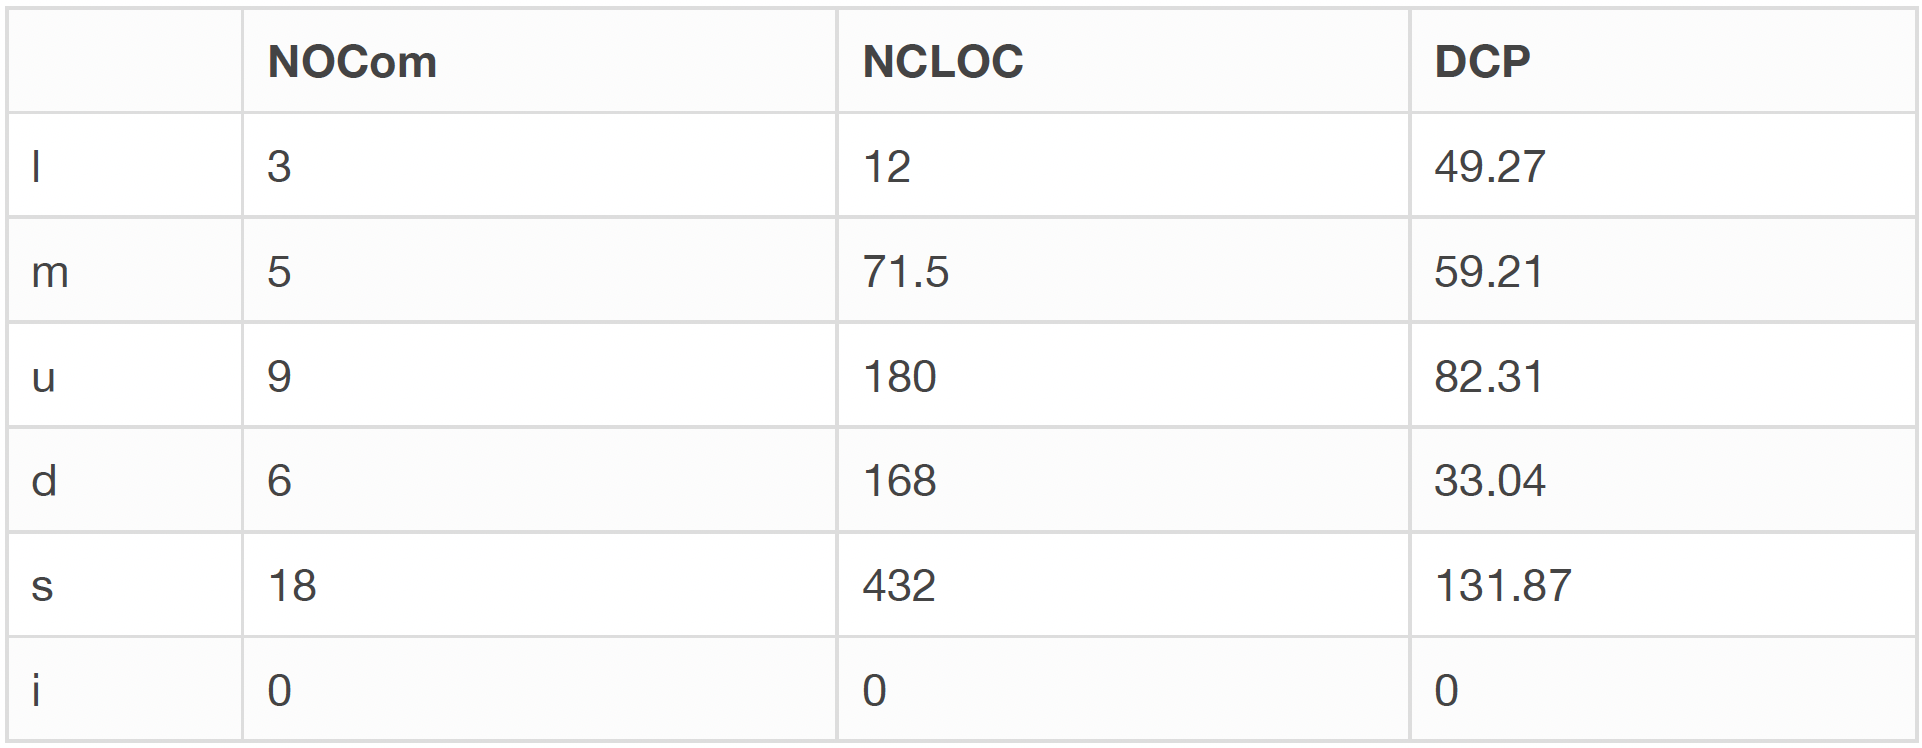
\includegraphics[scale=0.3]{T1_1.png}\\
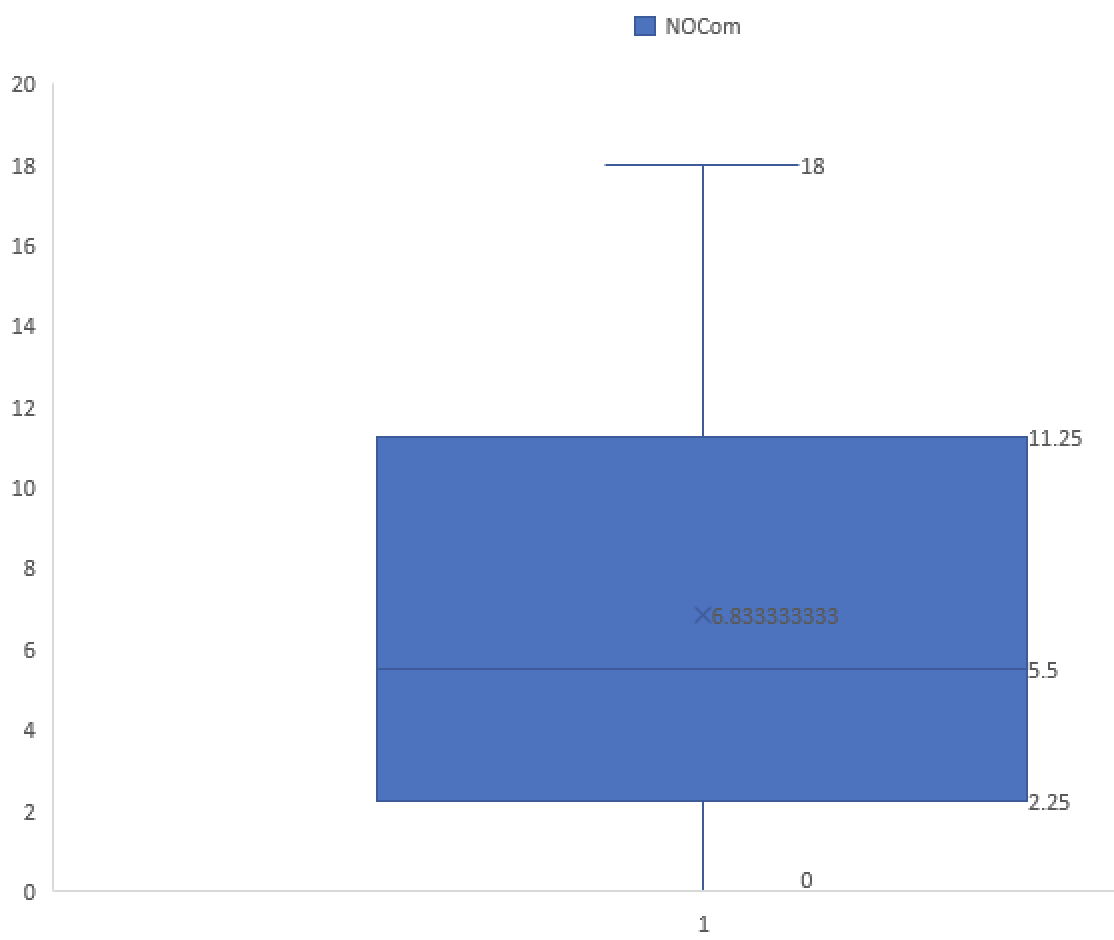
\includegraphics[scale=0.5]{NOCom.png}
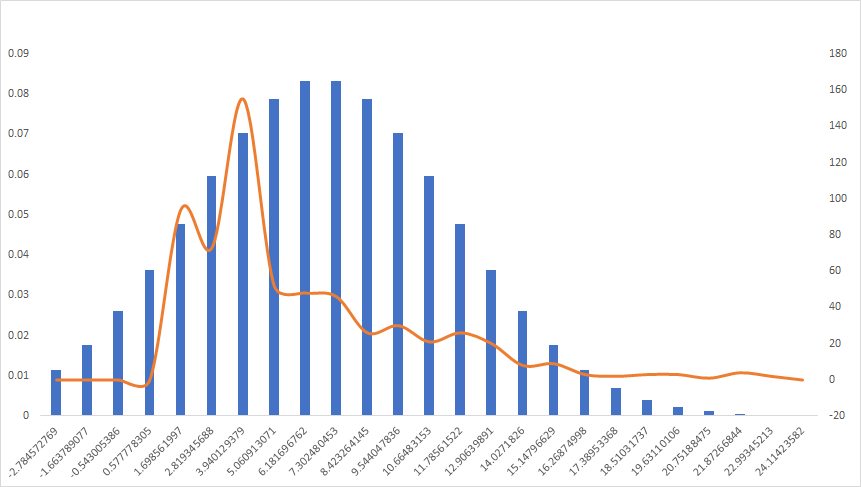
\includegraphics[scale=0.35]{T1_2.png}\\
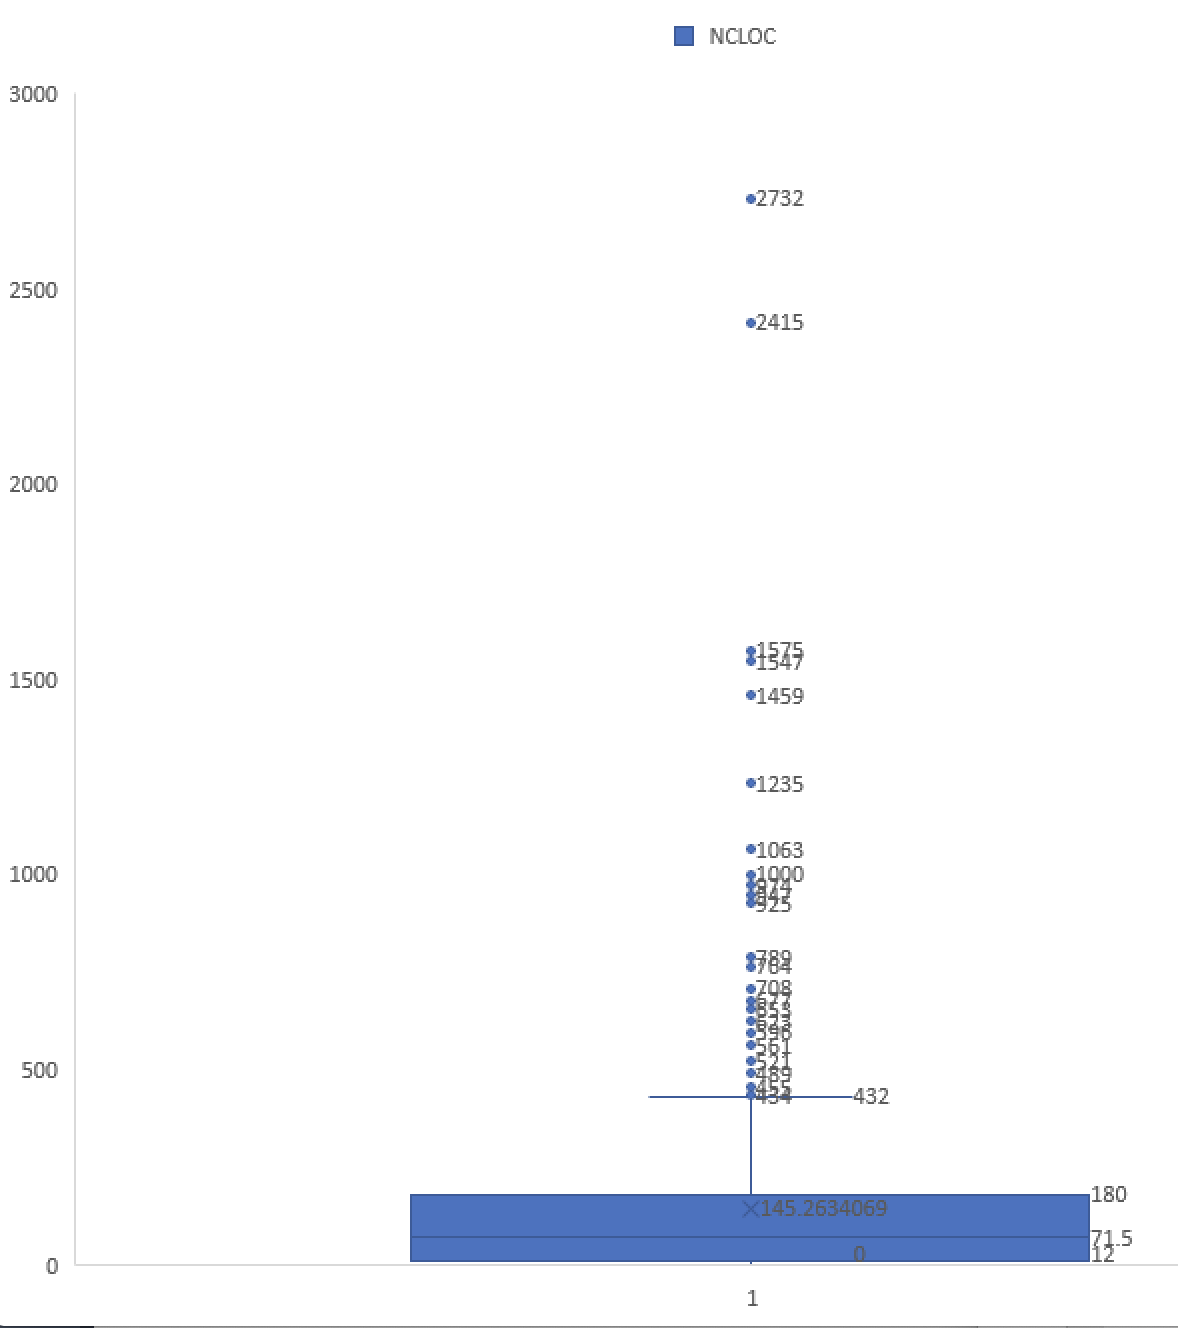
\includegraphics[scale=0.5]{NCLOC.png}
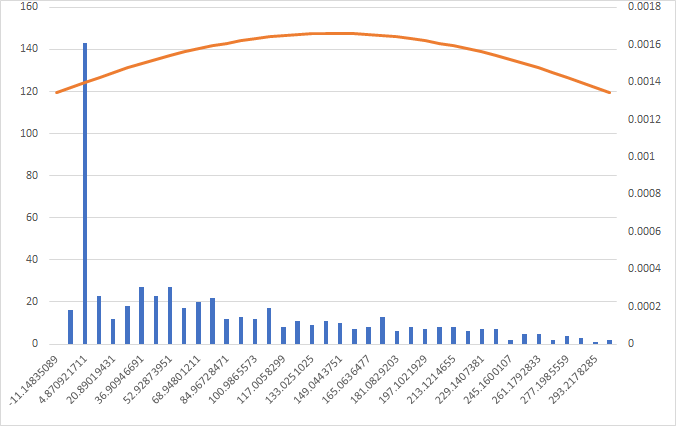
\includegraphics[scale=0.35]{T1_3.png}\\
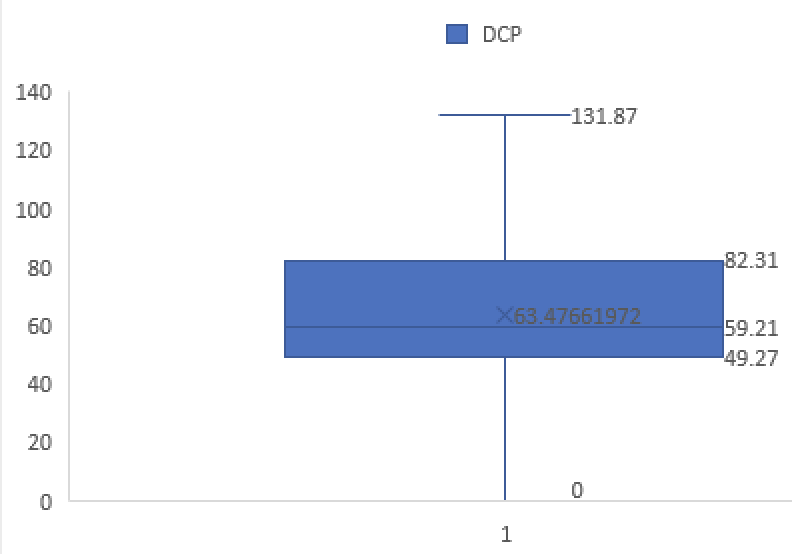
\includegraphics[scale=0.6]{DCP.png}
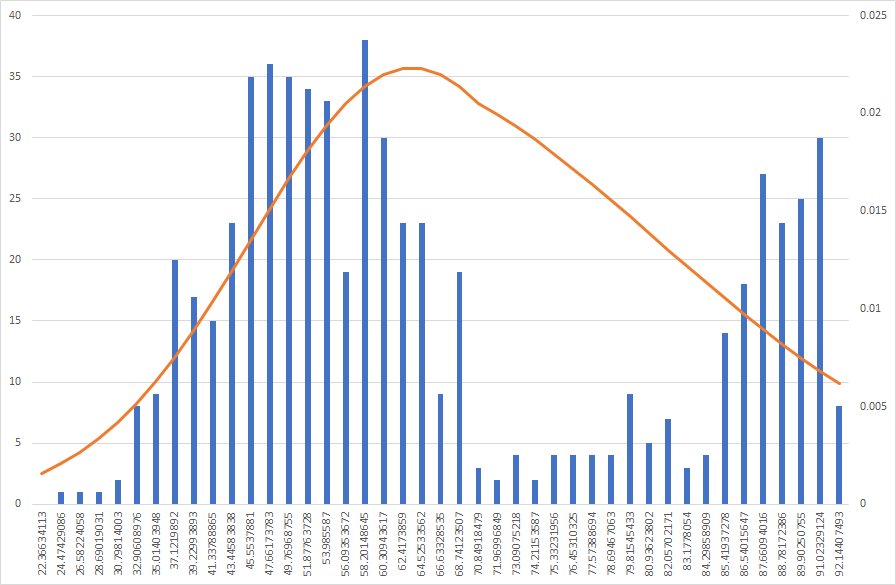
\includegraphics[scale=0.35]{T1_4.png}\\

Le tableau contient les informations nécessaires pour représenter la boîte à moustaches. À partir de la courbe de distribution, la distribution de NoCom n'est pas très proche de la distribution normale, tandis que la courbe normale de NCLOC est la meilleure, mais l'écart type est plus grand, la courbe normale de DCP est très proche de la courbe normale standard, et l'écart type est acceptable.\\


\section*{Tâche 2}\\

Coefficient de corrélation de Pearson (r):\\

r(NoCom, NCLOC) : 0.71457166 \qquad r(NoCom, DCP) : -0.487753\\

Coefficient de corrélation de rang de Spearman ($\rho$):\\

$\rho$(NoCom, NCLOC) : 0.7098611 \qquad $\rho$(NoCom, DCP) : -0.4267282\\

Courbe de régression:\\
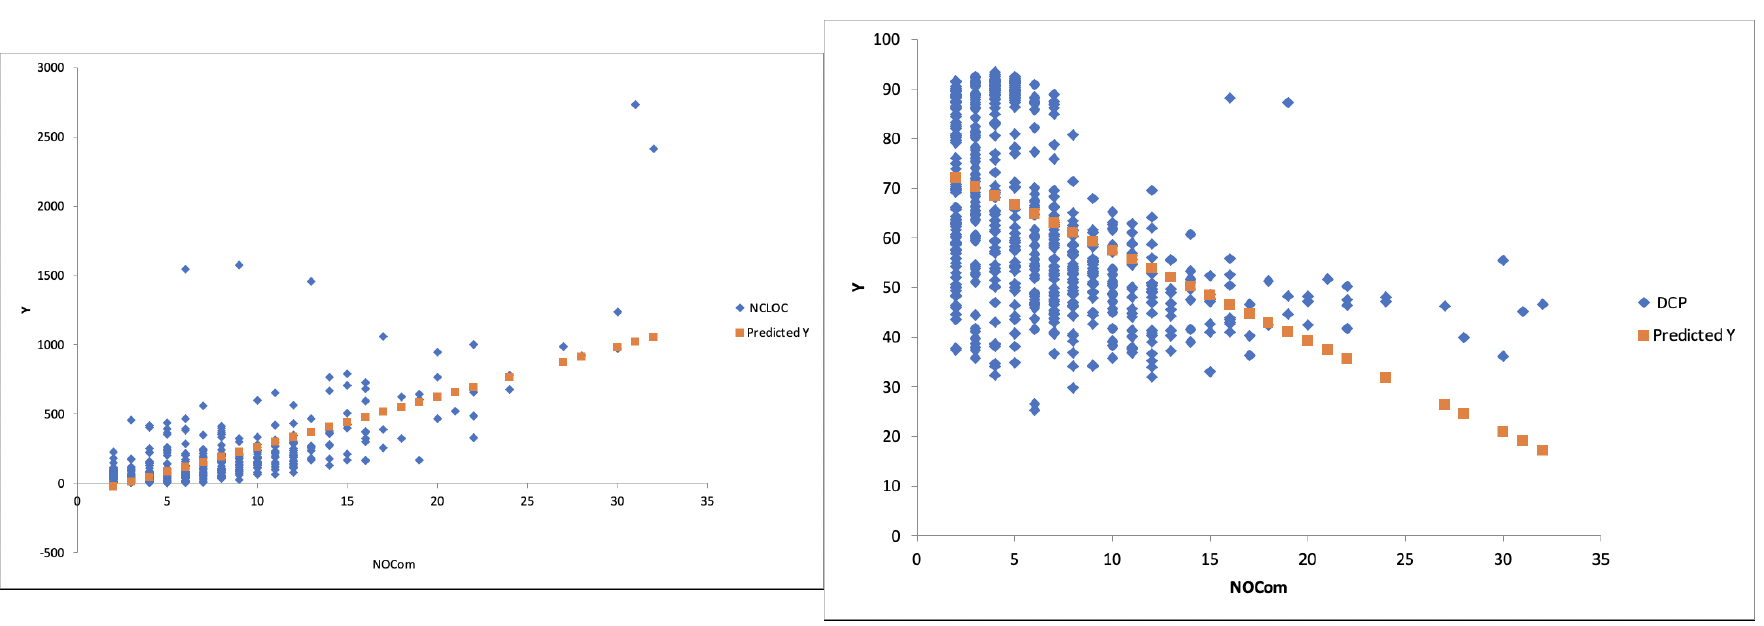
\includegraphics[scale=0.55]{T2.png}\\
Nous pouvons trouver à partir des trois indicateurs différents du coefficient de corrélation de Pearson (r), du coefficient de corrélation de rang de Spearman ($\rho$) et de la courbe de régression qu'il existe une forte corrélation positive entre NoCom et NCLOC, et une corrélation relativement forte entre NoCom et DCP Corrélation négative faible .





\section*{Tâche 3}\\
Evaluer l’hypothèse

\end{document}
